\documentclass[10pt,a4paper]{book}
\usepackage[utf8]{inputenc}
\usepackage{amsmath}
\usepackage{amsfonts}
\usepackage{amssymb}
\usepackage{epigraph}
\usepackage{graphicx}
\author{Alberto Rescia}
\newcommand{\code}[1]{\texttt{#1}}

\begin{document}

\chapter{The ATLAS Detector}
%\epigraph{Shrek: Ogres are like onions. \\
%Donkey: They stink? \\
%Shrek: Yes. No. \\
%Donkey: Oh, you leave 'em out in the sun they get all brown, start sproutin' little white hairs. \\
%Shrek: No. Layers. Onions have layers. Ogres have layers. You get it? We both have layers.}


%The ATLAS detector, much like a certain emotionally damaged ogre, has many layers. These layers serve the purpose of reconstructing, as much as physically possible, the full kinematics of a given final state. This is no easy task: with several billion bunch crossings per second, state-of-the-art technology\footnote{This was true in the '90s} is needed to meet the challenge. 

The ATLAS detector was designed for the purpose of reconstructing, as much as physically possible, the full kinematics of a given final state after a collision event at the Large Hadron Collider (LHC). This is no easy task: with several billion bunch crossings per second, state-of-the-art technology\footnote{This was more true in the '90s than it is today.} is needed to meet the challenge. 

In this chapter, we will describe the many layers which compose the ATLAS detector and illustrate how they come together to become the marvel of engineering that we know and love.

\section{The Large Hadron Collider}

Let us begin our journey from the underlying facility: the LHC. The LHC represents the largest particle accelerator ever built and currently in operation. It provides collisions for the four major experiments, ATLAS, CMS, LHCb and ALICE, along with a number of secondary experiments such as LHCf, TOTEM, MoEDAL and FASER. 

The LHC can be best described as an accelerator complex rather than a single collider. In fact, before protons (or heavy ions) are injected into the LHC, they are accelerated in stages in a number of steps which rely in part on previous colliders built at CERN. We shall briefly describe these stages.

First of all, protons are sourced from a flask of hydrogen gas. The gas is ionised with an electric field to isolate the protons. Next, the protons are accelerated with a linear accelerator. Up until 2020, this was the Linac 2, though later it was the Linac 4. This step brings the energy up to 50 MeV. Next, the protons are sent into the Proton Synchrotron Booster (PSB), which besides further accelerating the particles to 1.4 GeV also separates the proton beam into bunches. The protons are then injected into the Proton Synchrotron which brings the energy up to 26 GeV, followed by the Super Proton Synchrotron (SPS) which accelerates the protons to 450 GeV.

Lastly, the protons are injected into the LHC. This machine is a 27 km underground ring which is responsible for accelerating the particles to the final collision energy and maintaining that energy until collisions deplete the beam, at which point more protons are injected. 

The proton bunches are injected into two beam pipes and travel in opposing directions. At the four interaction points were the main experiments are located, the beam pipes cross every 25 ns allowing for collisions to occur.  

The main advantage of a circular collider is to maximise collision energy. During the first run of data taking (Run 1) from 2010-2013, the LHC collided protons at $\sqrt{s} = 7$ TeV or at $\sqrt{s} = 8$ TeV. In Run 2, from 2015-2018, protons were collided at $\sqrt{s} = 13$. Since 2022, Run 3 has been underway and protons are being collied at $\sqrt{s} = 13.6$ TeV. In the future, during Runs 4 and 5, the centre-of-mass energy may reach up to 14 TeV, depending on the magnets.

Figure \ref{lhc} shows the full accelerator complex at CERN, including all major and minor experiments currently underway.

\begin{figure}
    \centering
    \includegraphics[width=0.9\linewidth]{atlas/CCCv2019.png}
    \caption{The full accelerator complex at CERN \cite{Bartosik:2022cxq}.}
    \label{lhc}
\end{figure}

\subsection{Luminosity}

The luminosity is an important quantity to keep account of to know how many collisions have occurred. The instantaneous luminosity $L_{\text{instant}}$ is quantity given by some beam parameters which, together with the cross section $\sigma$ of some physics process, gives the rate for that process 

\begin{equation}
    \frac{dN}{dt} = \sigma L_{\text{instant}}.
\end{equation}

The instantaneous luminosity itself is given by

\begin{equation}
L_{\text{instant}} = \frac{N_1N_2fN_b}{4\pi\sigma_x\sigma_y}.
\end{equation}

Here, $N_1$ and $N_2$ represent the number of protons in the two bunches which collide, $f$ is the frequency of the beam, currently around 0.04 nHz, and $N_b$ is the number of bunches. $\sigma_x$ and $\sigma_y$ represent the beam width in the $x$ and $y$ directions.

If we integrate the instantaneous luminosity over time $L = \int L_{\text{instant}}dt$ we get the \emph{integrated luminosity}, which allows us to get the total number of collisions which have occurred $N$

\begin{equation}
    N = \sigma L.
\end{equation}
Figure \ref{lumi} shows the total integrated luminosity provided by the LHC during each year of operation, up to 2024. The results for individual experiments my vary slightly based on any dead time experienced by the detector.

\begin{figure}
    \centering
    \includegraphics[width=0.9\linewidth]{lumi}
    \caption{The total integrated luminosity provided by the LHC during each year of operation \cite{CERN}}.
    \label{lumi}
\end{figure}

Starting from 2030, the High-Lumi LHC programme is expected to increase the instantaneous luminosity delivered by the LHC by a factor 7.5. This is expected to deliever a total integrated luminosity of 3000 fb$^-1$ during Runs 4 and 5 \cite{ISSP}. This means that about 90\% of collisions are yet to be delivered, as of 2025!

\subsection{Pile-up}

Over time, the instantaneous luminosity at the LHC has increased. As it has increased, so too has the average pile-up.

Usually when proton bunches collide, at most 1-2 hard, head-on scattering events between protons will occur. These are the collisions which are the most interesting. However, there are often many underlying soft, lateral collisions between protons in the bunches. This is known as \emph{pile-up}.

In Run 1, the average pile-up $<\mu>$ per event recorded in ATLAS was roughly 20 collisions/interaction \cite{ATLAS:2017pfq}. This increased to $<\mu> = 33$ in Run 2 \cite{ATLAS:2023hxv}, and was as high as $<\mu> = 62$ in Run 3 during 2024 data taking. During Runs 4 and 5, pile-up is expected to increase to $\mathcal{O}(200)$ collisions/interaction.

%advantage of circular collider is to maxmise centre of mass energy
%this changes with different runs


\section{The ATLAS Detector}

The ATLAS experiment is a general-purpose experiment built to search for new physics phenomena. Back in the '90s and early '00s, these were principally believed to be the Higgs boson and supersymmetry (SUSY). Indeed, in 2012 ATLAS and CMS announced the discovery of the Higgs boson. The discovery of SUSY, however, never came to fruition. Regardless, the ATLAS precision physics programme provides valuable data which has been able to constrain models which extend the Standard Model beyond the energy ranges we can currently reach.

In this section, we will describe the design of the ATLAS detector during Run 2 to ascertain how it is capable of delivering such impressive results.

\subsection{The coordinate system}
Let us start by describing the coordinate system used at the experiment. 

ATLAS uses a right-handed cylindrical coordinate system. The $z$-axis is pointed along the beam, while the $x$-axis points towards the centre of the LHC ring and the $y$-axis points upwards towards the sky. 
In the transverse plane, polar coordinates $(r, \phi)$ are used. $\phi$ is the azimuthal angle around the $z$-axis, and $r$ gives the distance from the beamline in the $x-z$ plane.

For the sake of convenience, rather than $r$, the \emph{rapidity} $y$ is used, defined as

\begin{equation}
    y = \frac{1}{2}\ln\left(\frac{E + p_z}{E - p_z} \right)
\end{equation}

where $E$ and $p_z$ refer to the energy and the momentum along the $z$-axis of a given particles, respectively. At high energies, when $p \gg m$, the \emph{pseudorapidity} $\eta$ can be used equivalently

\begin{equation}
    \eta = -\ln\left(\tan(\theta/2)\right)
\end{equation}
where $\theta$ is the angle respect to the $z$-axis. The advantage of using $\eta$ rather than $y$ is that $\eta$ involves purely geometrical information, instead of four-momentum coordinates of a specific particle. 

Kinematics are closed in the transverse plane. This is due to the fact that, at high-energy hadron colliders, it is the partons which collide rather than the hadron itself. The partons are each carrying an unknown fraction $x$ of the total momentum, but conservation of momentum ensures that this quantity is conserved in the transverse plane.

\subsection{Magnets}

The magnetic field is a key feature of the detector since it allows for the measurement of particles' charge and momentum through their deflection via the Lorentz force. There are two magnet systems present at ATLAS. The first is a 2 T solenoidal magnetic field the along the $z$-direction. The second is a toroidal magnetic system placed on the muon spectrometer, which coincides with outermost part of the detector. There is one toroidal magnet in the central barrel and two in the end-caps. In the central barrel, the toroidal magnet produces a field of 1 T, while in the end-caps the field produced is of 0.5 T. The acronym ``ATLAS'' originally stood for ``A Toroidal LHC ApparatuS''. The toroidal magnets therefore can be seen as the defining feature of the detector. The magnetic field lines within the ATLAS detector are show in Figure \ref{magnet}.

\begin{figure}
    \centering
    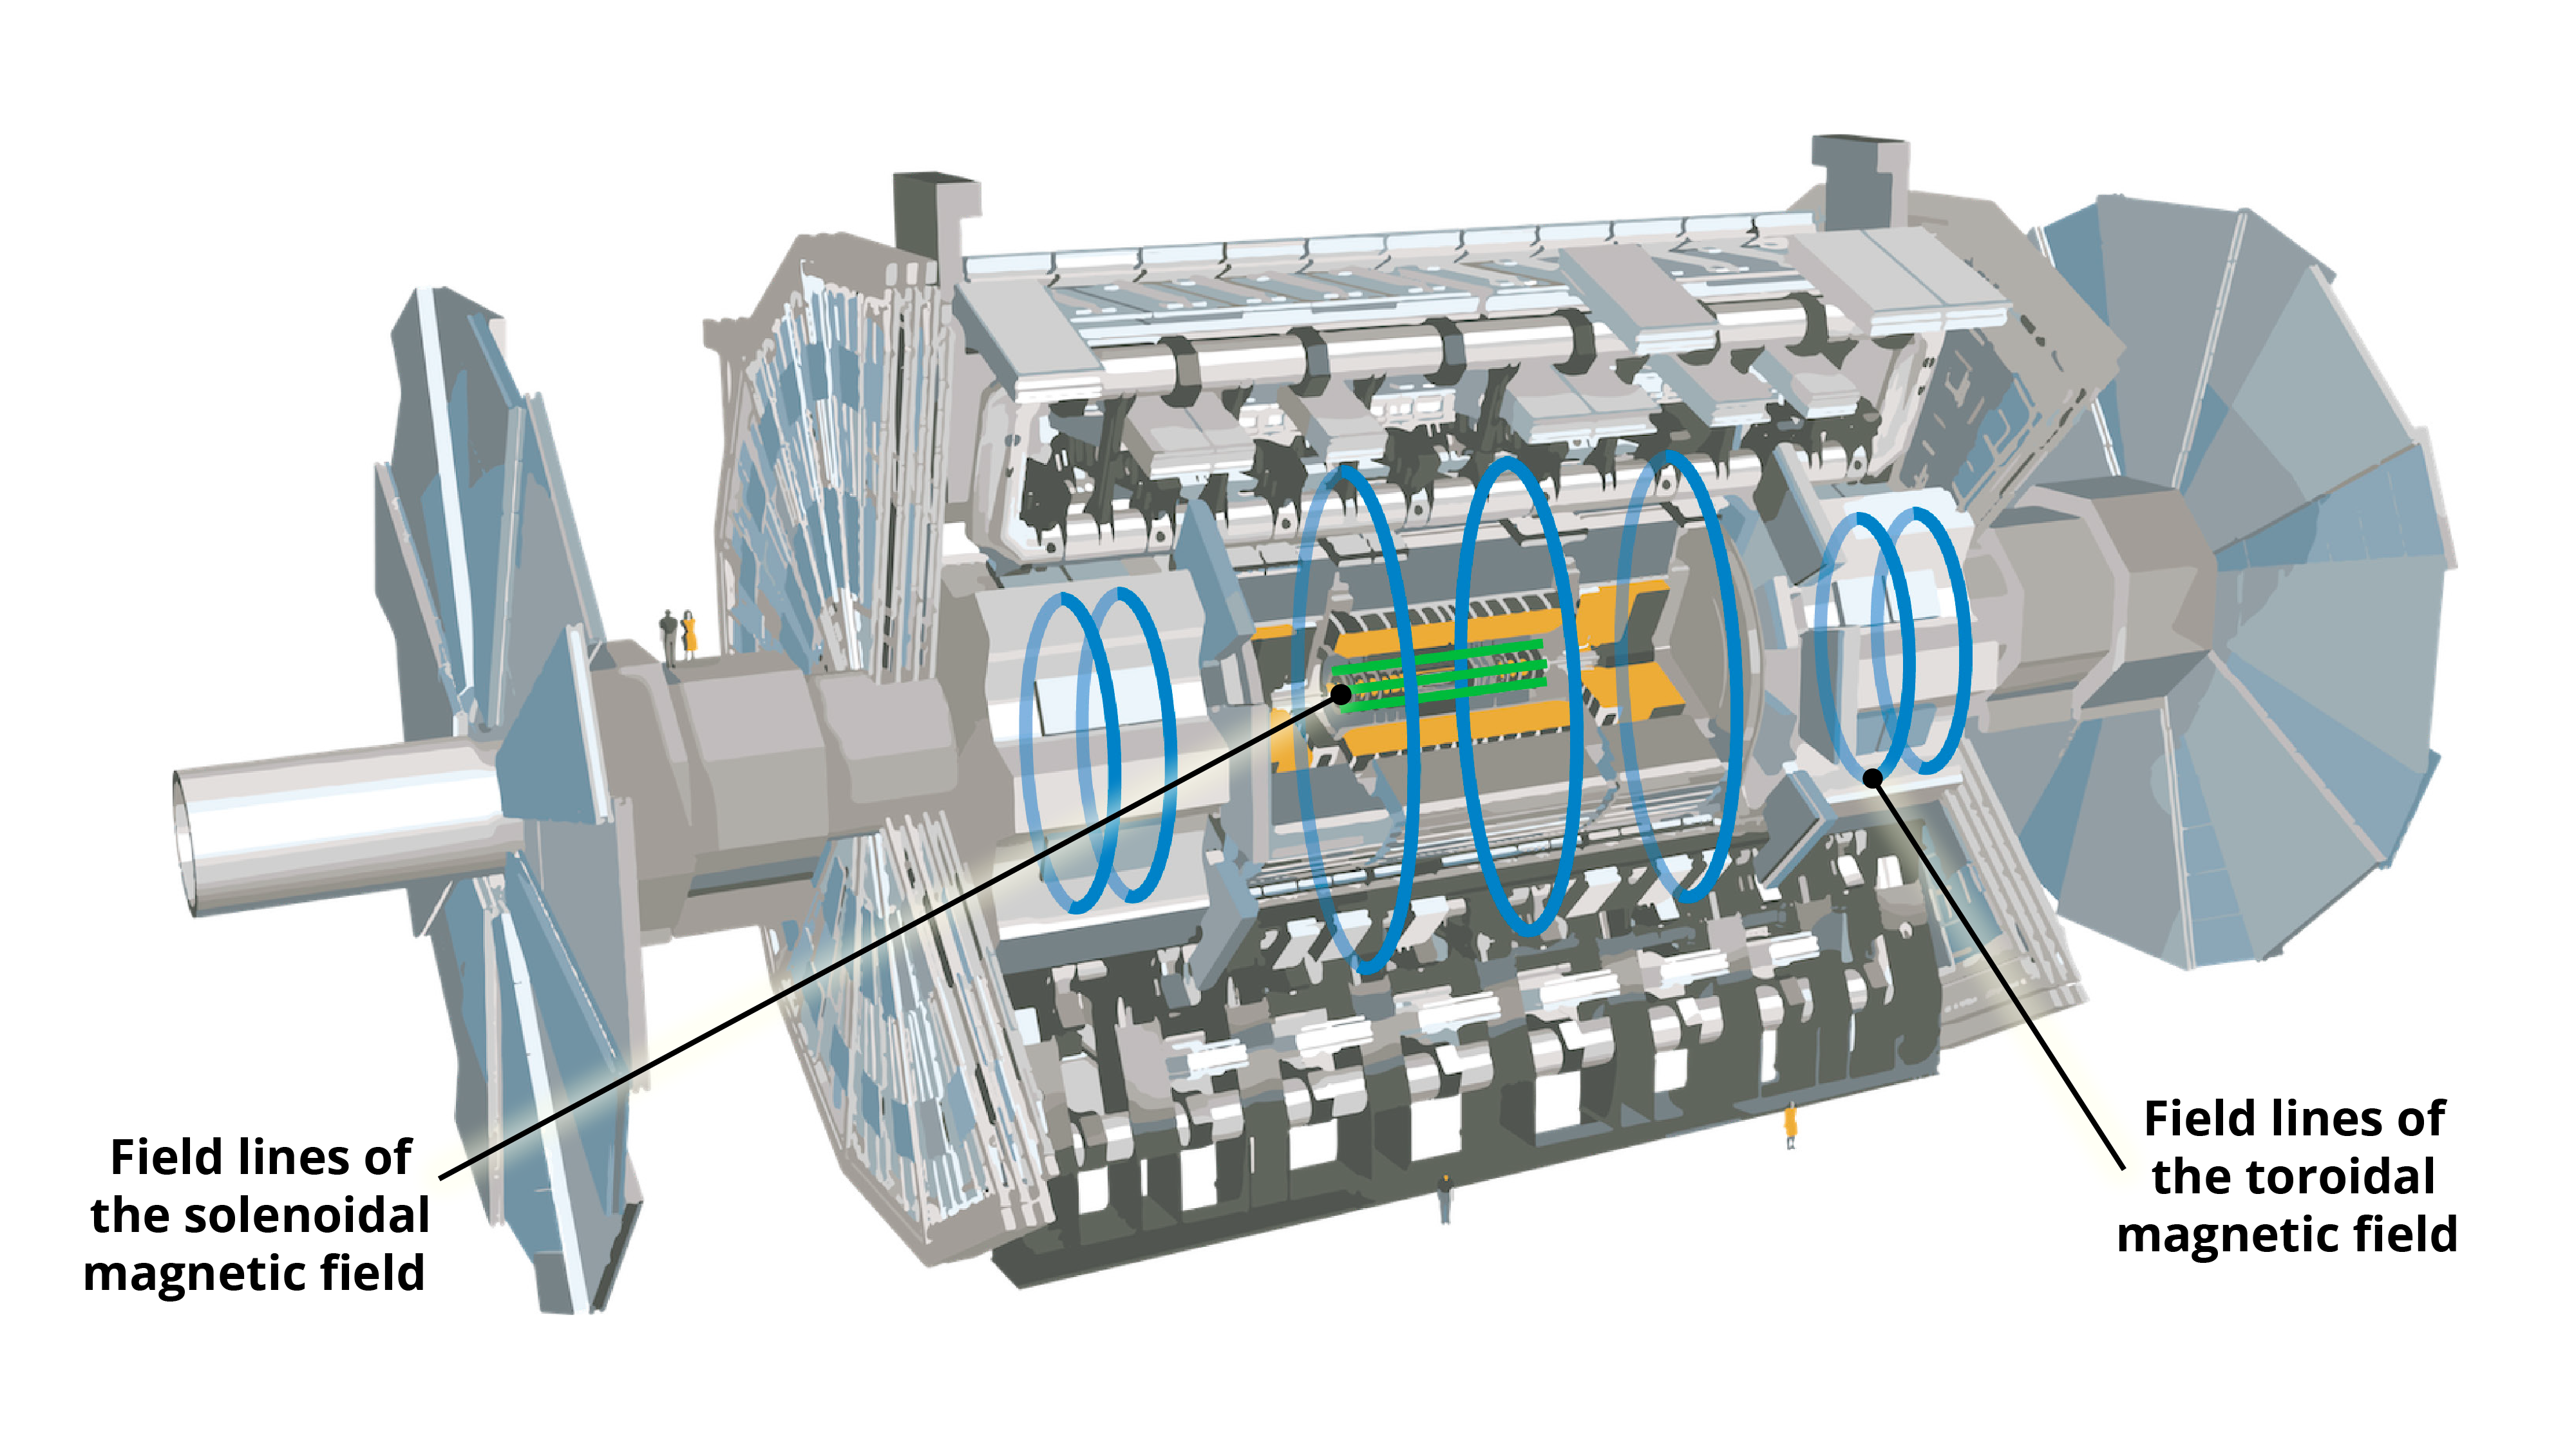
\includegraphics[width=0.8\linewidth]{atlas/magneticfield.png}
    \caption{The solenoidal and toroidal magnetic fields generated within the ATLAS detector \cite{RodriguezVera:2770604}.}
    \label{magnet}
\end{figure}

\subsection{Inner detector}

The innermost layer of the ATLAS detector is known as the \emph{Inner Detector} (ID). Covering a range up to $\vert \eta \vert < 2.5$, it is designed to track charged particles as they moved through the detector, deviated by the magnetic field. The presence of the magnetic field allows quantities such as the charge and momentum of the particle to be determined.  

The ID is composed of three subsystems:  the Pixel Detector, the SemiConductor Tracker (SCT) and the Transition Radiation Tracker (TRT). The ID and its subsystems, which we describe below, are shown in Figure \ref{id}.

\begin{figure}
    \centering
    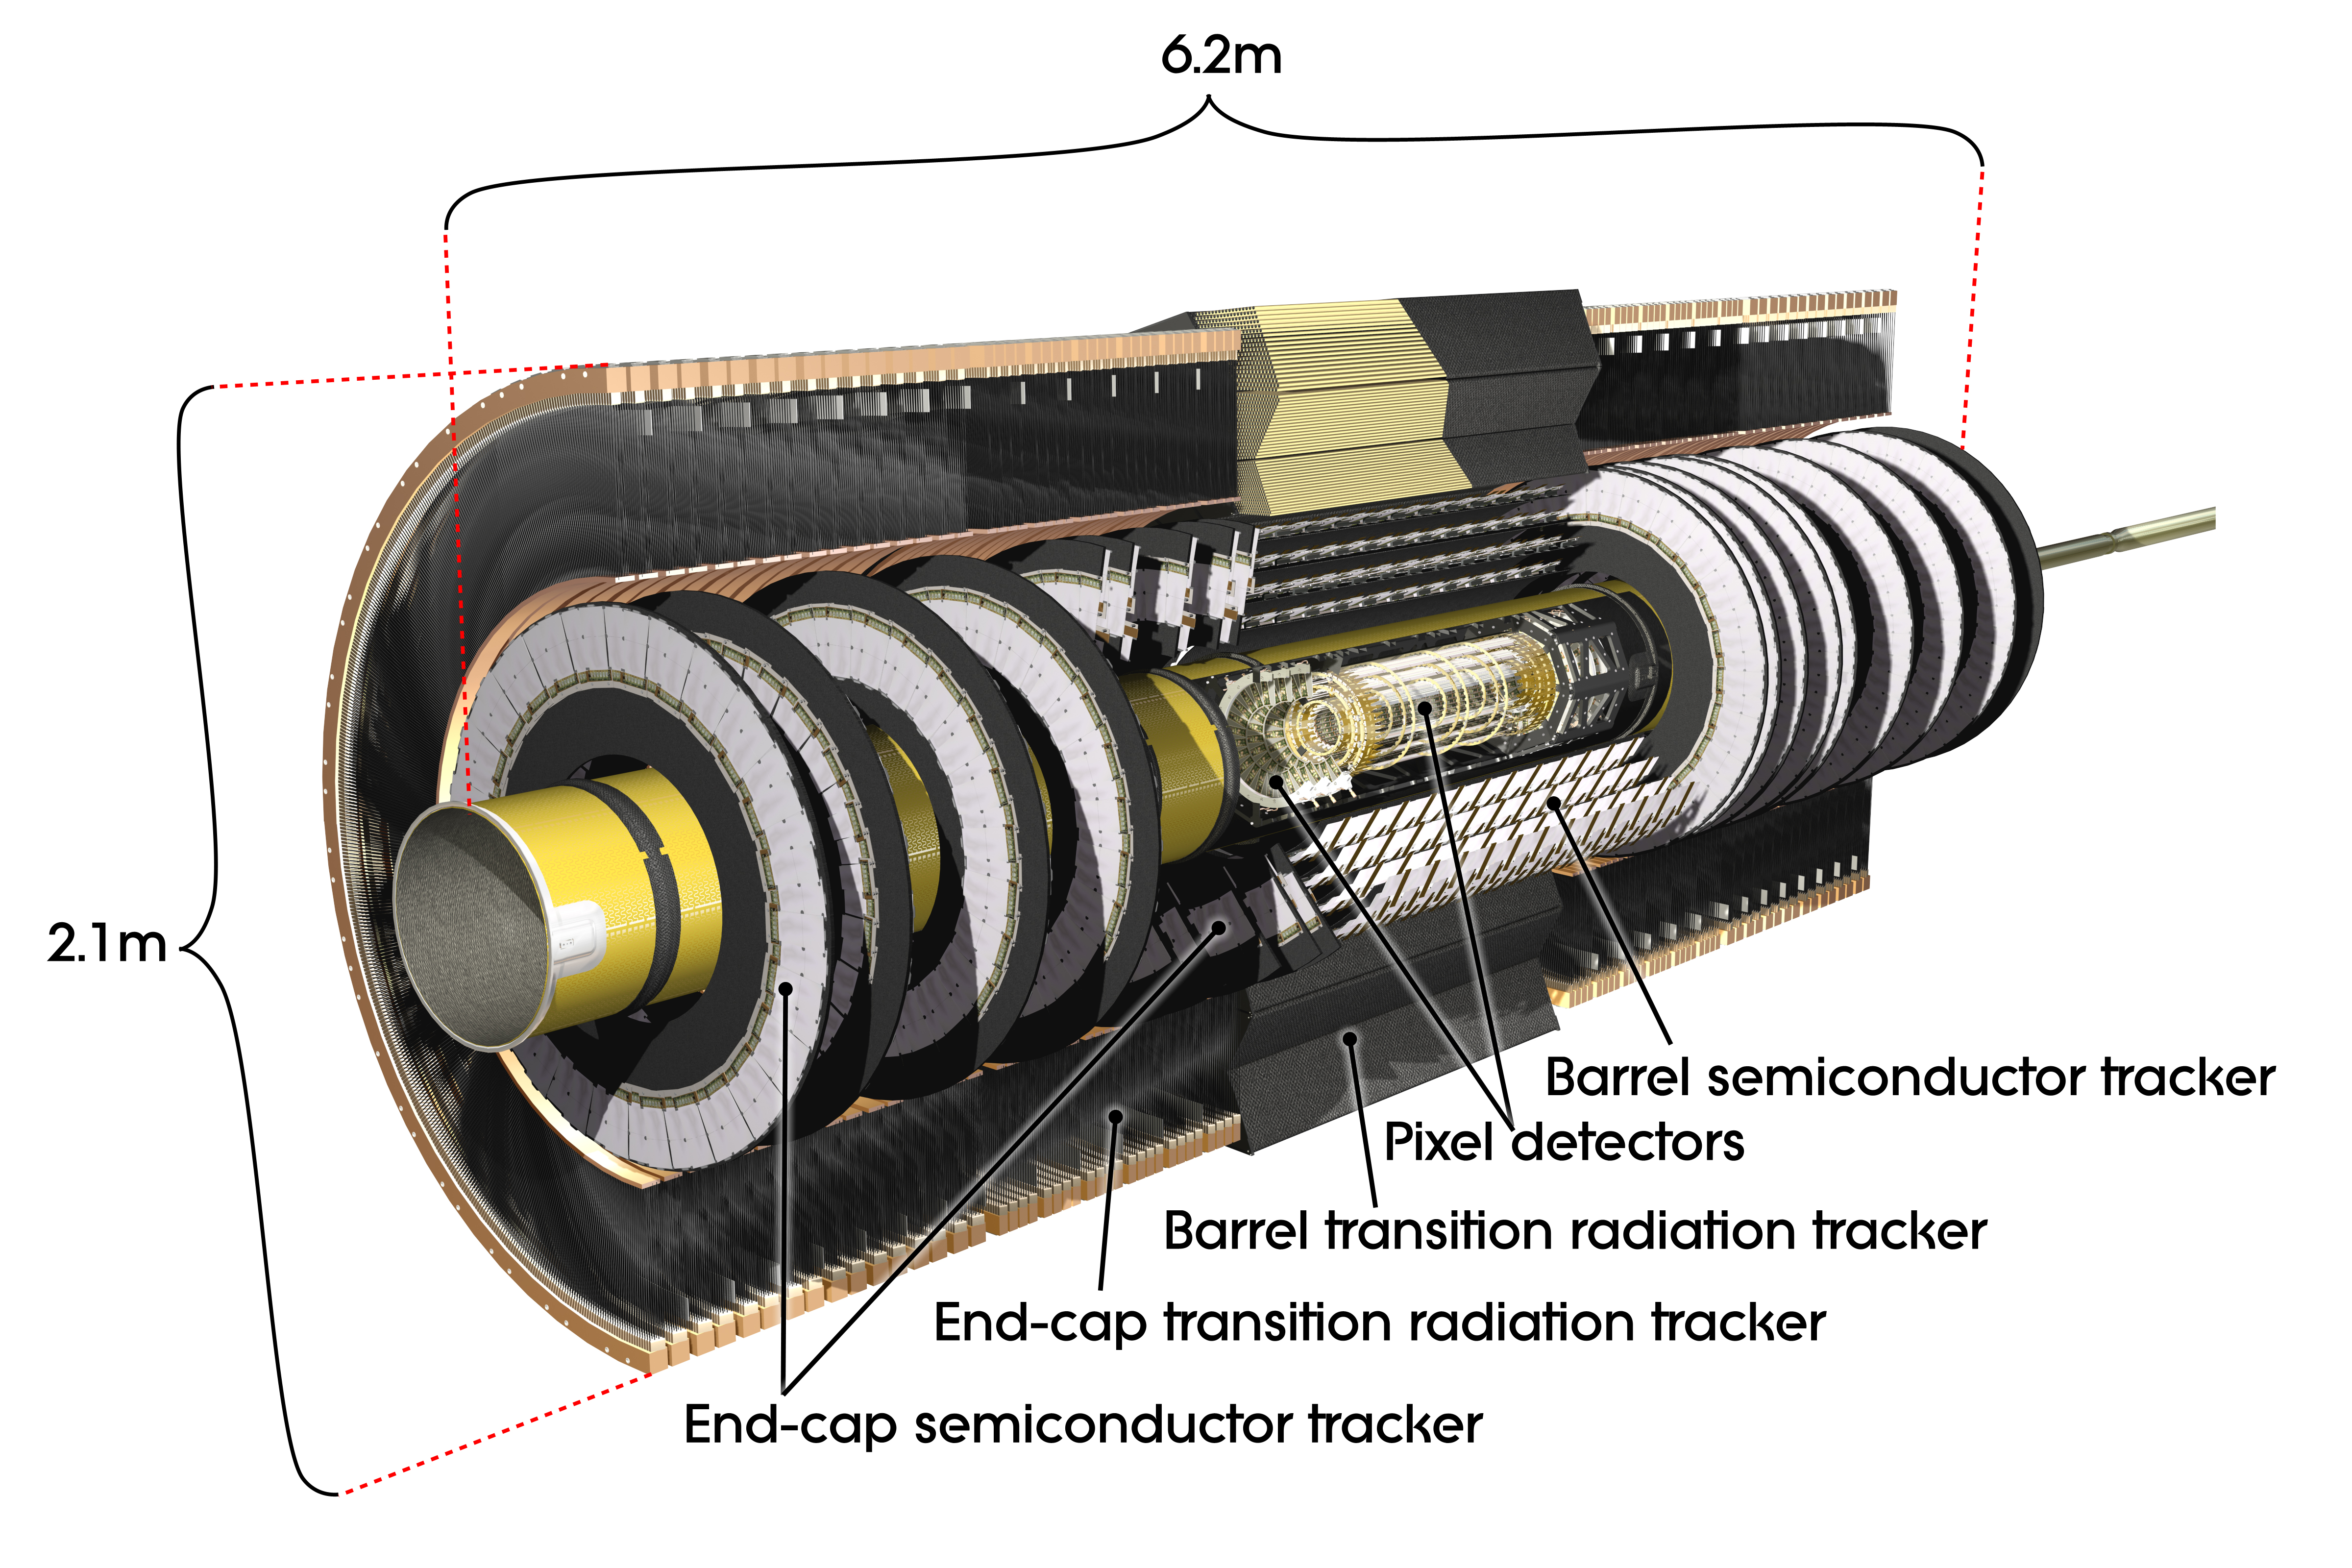
\includegraphics[width=0.8\linewidth]{atlas/innerdetector.jpg}
    \caption{The Inner Detector and all of its subsystems \cite{Pequenao:1095926}.}
    \label{id}
\end{figure}

\subsubsection{Pixel Detector}
The silicon Pixel Detector is the closest to the beamline -- just 3.3 cm away -- and thus has been designed to provide the highest granularity. It consists of four cylindrical layers, as well as two end-caps with 3 layers each. 
The innermost layer of the central barrel of the subdector is known as the Insertable B-Layer (IBL). This part of the Pixel Detector has the highest granularity at 50~$\mu$m in the transverse plane and 250~$\mu$m along the $z$-axis. The other three layers also have a resolution of 50~$\mu$m in the transverse plane, but a wider 400~$\mu$m along the $z$-axis. Thanks to the geometry of the detector, this leads to a total resolution of 8-10 $\mu$m in the transverse plane and 40-115 $\mu$m in the $z$ direction. On average, a charged particle will leave 4 hits in the Pixel Detector. 

\subsubsection{SCT}
The SCT is also a silicon detector, though it is based on strip technology rather than pixels. Each strip has a length
of 80 $\mu$m, and they are combined into modules composed of two sensors placed at an angle of 40 mrad with respect to each other. In this way, a module allows for two-dimensional reconstruction of the direction of the charged particle. Strip modules are arranged into four cylindrical layers and two end-caps with 9 layers of modules each. The SCT accuracy is required to be $\sigma(r\phi) = 17 \; \mu\text{m}$ and $\sigma(rz) = 580 \; \mu\text{m}$ \cite{Sandaker:1089261}.

\subsubsection{TRT}
The TRT is the outermost part of the ID. It is a gaseous detector composed of cylindrical (straw) tubes with a diameter of 4 mm and is characterised by an intrinsic accuracy of 130 $\mu$m per straw.  The TRT is capable of providing particle-identification. The empty space between the straws is filled with polymer fibres. As a particle traverses the boundary between the media, it emits radiation. The frequency of the the radiation depends on the Lorentz boost of the emitting particle $\gamma \sim E/m$. As such, the TRT can distinguish particles of different masses, provided they have the same momenta. Generally, this equates to distinguishing electrons from pions within the momentum range $1-100$ GeV$^2$.  

\subsection{Calorimeters}

ATLAS has two calorimeters: the Electromagnetic Calorimeter (ECAL), designed principally to detect energy deposits by electrons, positrons and photons, and the Hadronic Calorimeter (HCAL), designed to detect energy deposits by hadrons. 

The calorimeters are nearly hermetic, covering the full span of $\phi$ and $\vert \eta \vert < 4.9$, in order to contain as much of the energy of the event as possible. Both calorimeters are \emph{sampling calorimeters}. They feature an active layer where the energy is deposited, and a high atomic number passive layer which induces showers. The calorimeters measure only a fraction of the energy deposited, which is however proportional to the total energy of the particle responsible for the deposit. 

The ECAL uses lead as a passive material and liquid argon (LAr) as the active material. The HCAL, on the other hand, uses varying materials. In the end-cap calorimeters, liquid argon is used as the active material. The former, however uses copper and tungsten as passive materials, while the latter uses just copper. In the barrel, the tile calorimeter uses steel as a passive material and plastic scintillator as the active material. 

The region between the barrel and end-cap calorimeters is known as the \emph{crack region}. It is found between $1.37 < \vert \eta \vert < 1.52$. As this region has a particularly high amount of passive material, electrons and photons at these pseudorapidities are often excluded from analyses \cite{Ducu:2024sgj}.

Both electromagnetic and hadronic showers have a characteristic length. In electromagnetic showers, this is $X_0$, or the length at which the shower energy is depleted by a factor $1/e$. In hadronic showers, the characteristic length is the average distance travelled by a hadron between nuclear interactions $\lambda$. In these units, the ECAL has a depth $X_0 = 22$ and the HCAL has a depth $\lambda = 10$. Therefore, both are able to contain a majority of the energy deposited.

The ATLAS calorimeters are represented in Figure \ref{calo} .

\begin{figure}
    \centering
    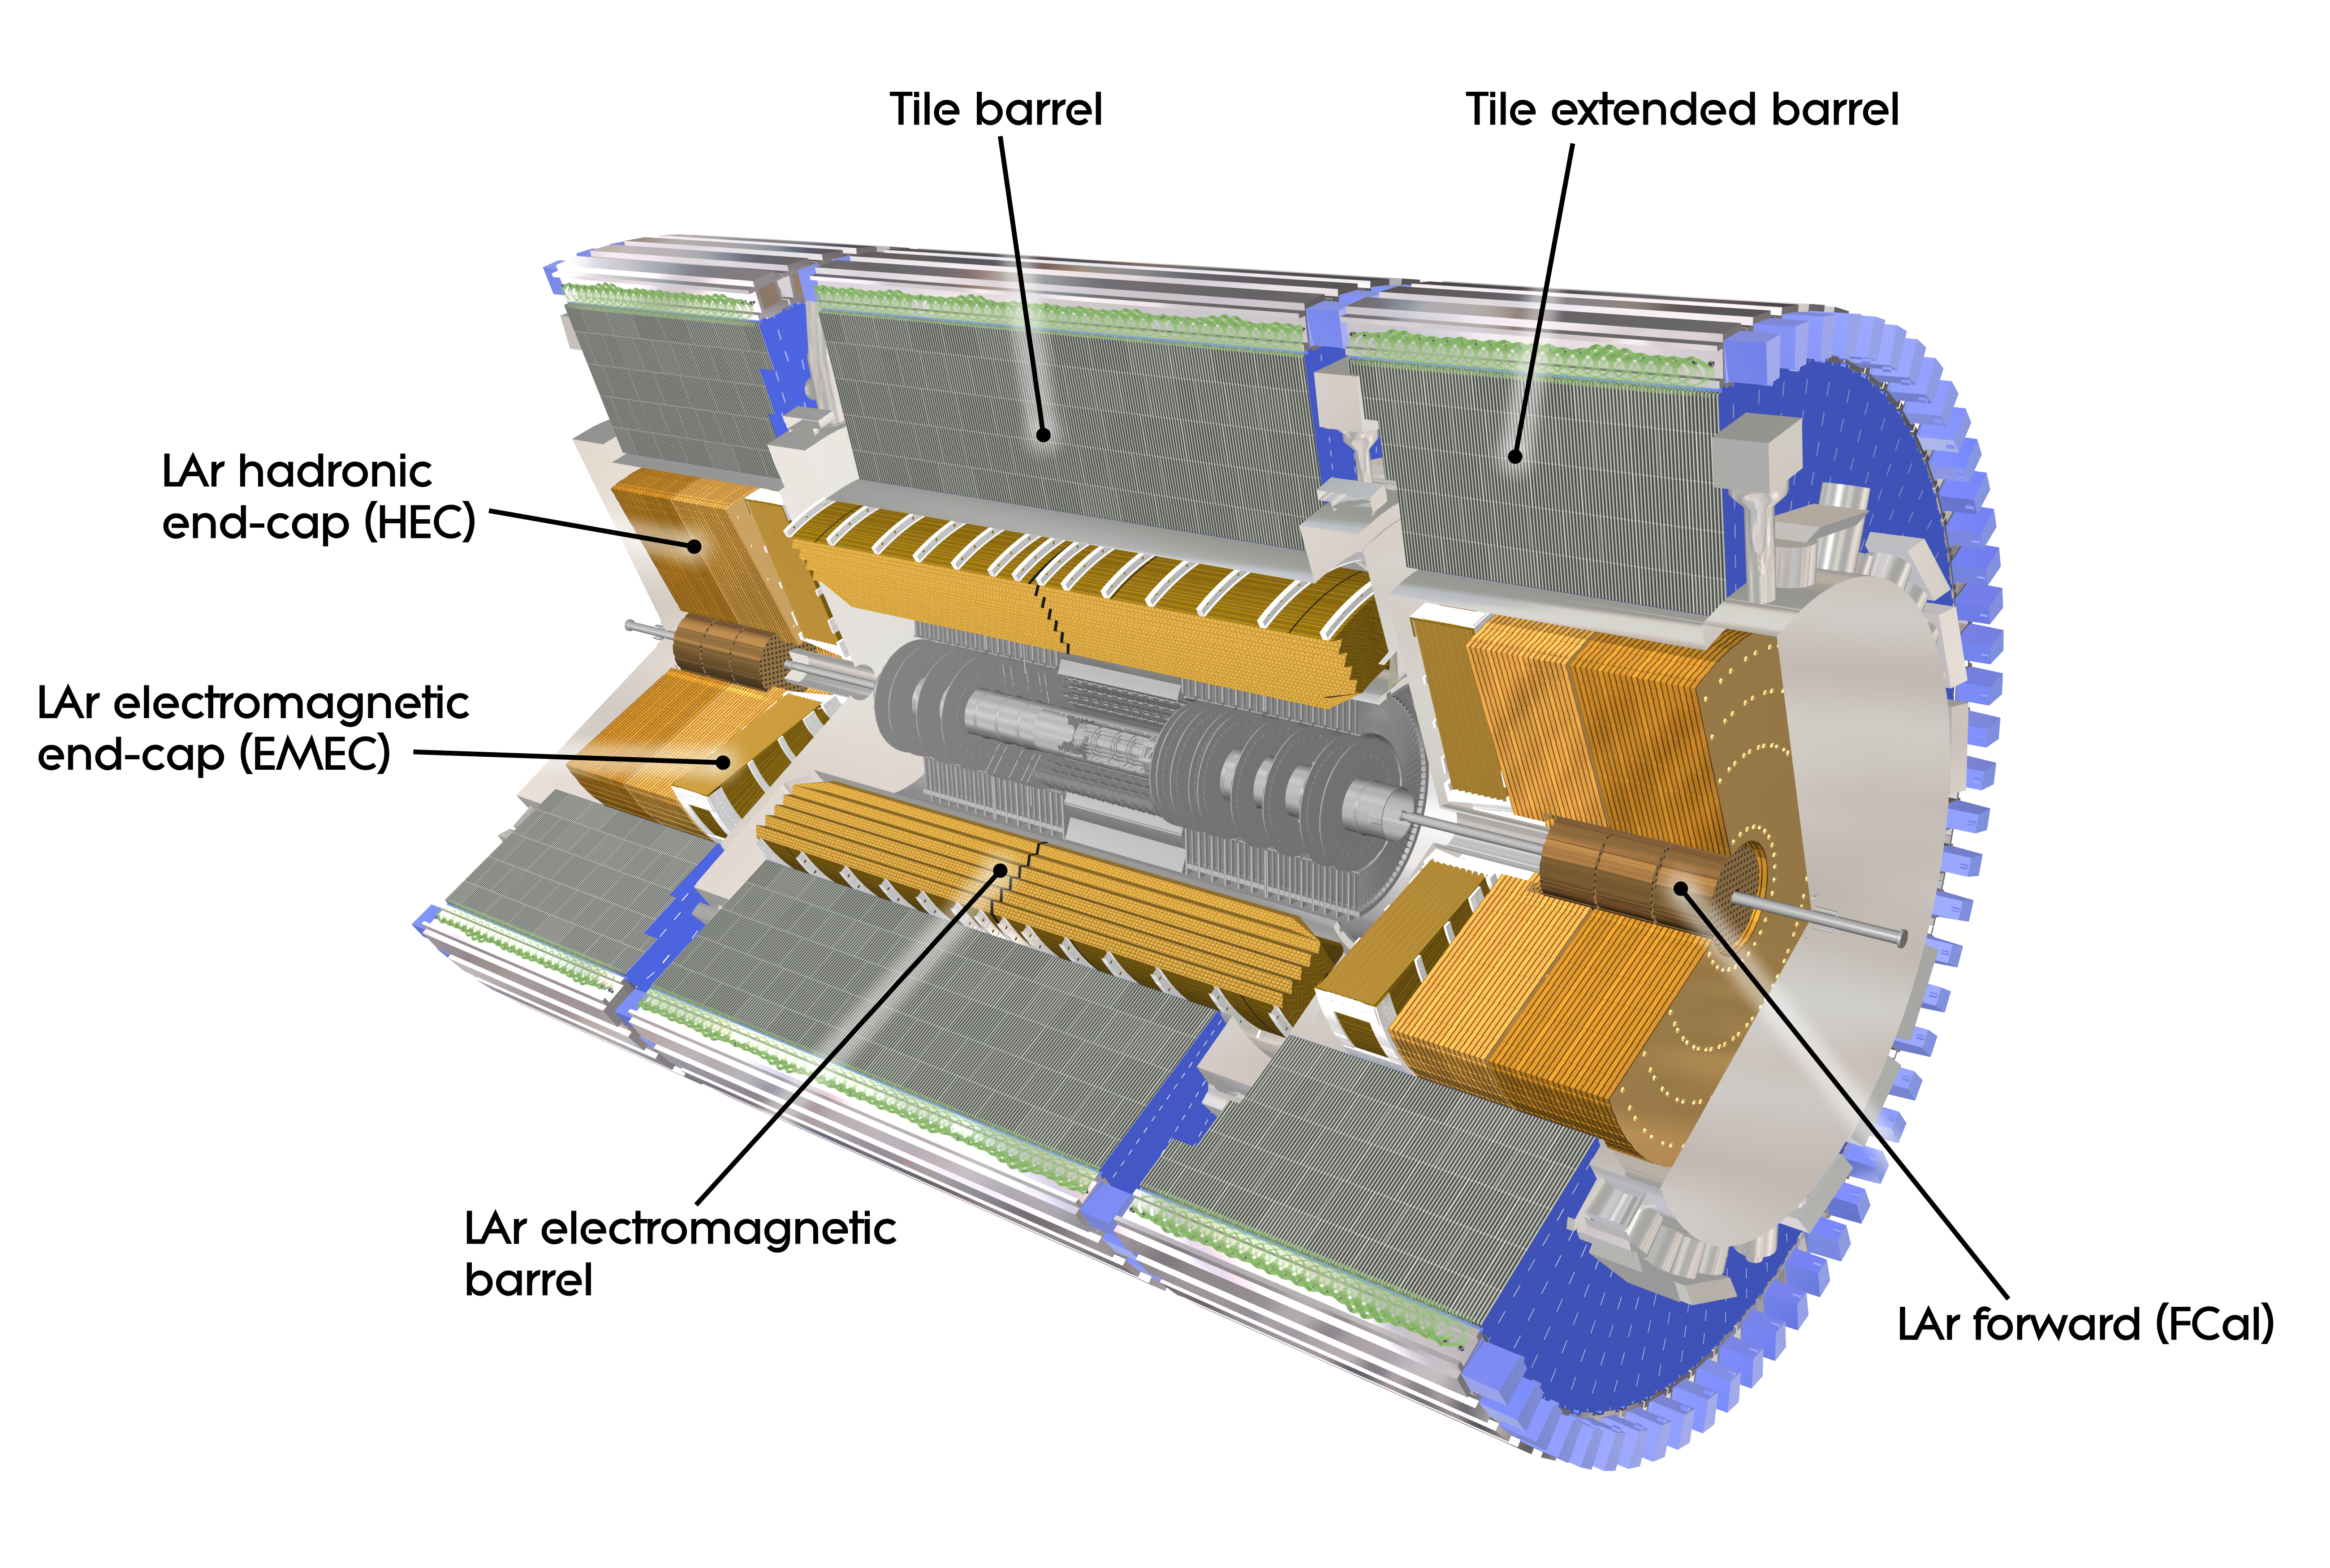
\includegraphics[width=0.8\linewidth]{atlas/calo.jpg}
    \caption{The ATLAS ECAL and HCAL systems \cite{Pequenao:1095927}.}
    \label{calo}
\end{figure}

\subsection{Muon spectrometer}

Muons produced by colliders are typically minimum ionising particles; they deposit little energy in the detector and are able to fly through and escape. Thankfully, they do deposit \emph{some} energy, appearing as tracks which are then reconnected to hits in the outermost layer of the detector: the muon spectrometer (MS). 

The Monitored Drift Tube (MDT) allows for precision tracking. It spans a region up to $\vert \eta \vert < 2.7$ and is composed of multiple layers. In the central region, up to $\vert \eta \eta < 2.0$, the MDT provides a resolution of 35 $\mu$m. In the high occupancy region, between $2.0 < \vert \eta \vert < 2.7$, the Cathode Strip Chambers (CSCs) provide coverage. These are multi-wire proportional chambers which provide a resolution of 60 $\mu$m in the $r$ direction and 5 mm in the $\phi$ direction. 

The muon spectrometer also features a built-in trigger system . Three layers of Resistive Plate Chambers (RPCs) are used in the central barrel region and 3-4 layers of Thin Gap Chambers in the end-cape regions. These two systems provide a hardware trigger by detecting the coincidence of the hits in the different layers when a muon passes through the detector. They also allow a measurement of the trajectory of the particle.

The muon spectrometer in its entirety is shown in Figure \ref{muon}.

\begin{figure}
    \centering
    \includegraphics[width=0.7\linewidth]{atlas/muon.jpg}
    \caption{The ATLAS muon spectrometer \cite{Pequenao:1095929}.}
    \label{muon}
\end{figure}

\subsection{Trigger}
The rate of collisions at the LHC is 40 MHz. As such, an extraordinary amount of data is produced, more than we are capable of storing. It is therefore necessary to put in place a trigger system to select and save only the most interesting collisions.
The ATLAS trigger system is composed of the Level 1 Trigger (L1) and the High Level Trigger (HLT). The L1 Trigger is hardware based system which, based on signatures in the MS and calorimeters, decides if an event contains high-$p_t$ particles. It reduces the rate of events to roughly 100 kHz. These interesting events pass are saved in a buffer, and are then fed to the HLT, which operates on a dedicated farm. The HLT has access to information from the entire detector as well as regions of interest identified by the L1 Trigger. It uses software to further skim the number of events, down to a rate of 1.5 kHz. These then get written to disk as data.

\subsection{Detector operations}
It takes a dedicated team to run the ATLAS detector. During data taking periods, typically from March-October, hordes of people are responsible for monitoring each subsystem in real time, both day and night. Some may be in the control room, ensuring that the detector is functioning as expected. Others are behind the scenes, updating trigger keys based on information coming from the LHC, ensuring each subsystem of the detector is ready for the plan of the day, and others still are monitoring data quality to identify that the events saved are indeed useful.

Personally, I was involved in Run Control and Trigger Operations. I was responsible for monitoring detector dead-time, warnings and errors in real-time and reacting to them appropriately. I also monitored trigger rates to anticipate any problems in the various detector subsystems, and adjusted the triggers to account for the decrease in instantaneous luminosity as the protons in the beam were exhausted, and prepared the triggers and detector for each new fill from the LHC. 

\subsection{Putting it all together}
The combination of various subsystems allow for the identification of the majority of particles that pass through the ATLAS detector.

Charged particles are tracked in the ID. Muons will also produce hits in the MS, allowing for the identification of tracks corresponding to muons. Electrons and positrons will deposit there energy in the ECAL. Pions, kaons and other charged hadrons will instead deposit their energy in the HCAL. Photons will only deposit energy in the ECAL. Neutrinos will pass through the detector without leaving a trace, appearing only as missing transverse energy $E_T^{miss}$. The signatures that various particles leave in the detector are schematically represented in Figure \ref{signatures}. The detector as a whole is represented in Figure \ref{detector whole}. 

The hits (or lack thereof) produced in the different layers allows for the construction of what is known as \emph{physics objects}. These are objects such as electrons, photons, muons, which directly correspond to particles, though they can also be more abstract concepts such as tracks, $E_T^{miss}$ and jets. Data analysis is carried on physics objects, and calibration ensures that any detector effects are corrected for before carrying out the analysis. 

\begin{figure}
    \centering
    \includegraphics[width=0.98\linewidth]{atlas/atlas_particles.png}
    \caption{The signatures left by different types of particles in the ATLAS detector~\cite{Mehlhase:2770815}.}
    \label{signatures}
\end{figure}

\begin{figure}
    \centering
    \includegraphics[width=0.85\linewidth]{atlas/detector.jpg}
    \caption{The ATLAS detector with all subsystems. \cite{Pequenao:1095924}.}
    \label{detector whole}
\end{figure}

%citations throughout text ch 2
%object reconstruction -> move
%fix images ch 1 -> higgs potential
%corrections ch 4
%unico pdf

\section{Object reconstruction}

In this section, we will discuss how the relevant physics objects for this thesis are reconstructed. These are the basis for the selections for the analysis described in Chapter sadlòkfjasd. 

\subsection{Tracks}
Tracks are formed by matching hits in the different layers of the ID. Two algorithms are used for reconstruction. The first is an inside-out algorithm which reconstructs tracks starting from any series of 3 or more hits along the same axis in the various layers of the Pixel and SCT detectors. The track is then extrapolated to the end of the SCT detector, accounting for the magnetic field. Multiple candidates are considered in cases where ambiguity is present; the final selection is made based criteria such as the fit quality or the number of missing hits, which would penalise the candidate in question. The tracks which pass this step are extended to the TRT and combined with the hits registered in that subdetector. 
To cross-check the result of the track fitter, a complementary outside-in algorithm is run, known as back-tracking. This time, the algorithm starts from hits in the TRT and gradually adds hits in the silicon layers to form tracks. This algorithm is also able to trace tracks coming from photon conversions, decay chains of long-lived particles such as the $K_S$, and other charged particles produced in a way which would not produce hits in the silicon layers. 

\subsubsection{Track coordinates}
In the ID, tracks are immersed in a solenoidal magnetic field, leading to helicoidal trajectories. It is thus useful to use a helicoidal coordinate system to define the trajectory in space. The parameters used to define the trajectory are $(d_0, z_0, \phi, \theta, q/p)$. These correspond to, in order, the transverse ($d_0$) and longitudinal ($z_0$) impact parameters, or the distance between the closest point of the trajectory of the track and a reference point in the transverse plane or along the $z$-axis; the azimuthal ($\phi$) and polar ($\theta$) angles of the track at the point of closest approach to the reference point; and the ratio ratio q/p of the charge of the reconstructed track divided by the magnitude of its momentum. The reference point is usually taken to be the beamspot position, or the average point of $pp$ interactions.

\subsubsection{Track quality}
Tracks used for analyses must be within the acceptance of the ID ($\vert \eta \vert < 2.5$) and have a $p_t > 500$~MeV. Additional quality requirements can sometimes be placed to filter out fake tracks. Examples of these are
\begin{itemize}
    \item \textbf{Loose Track Quality:} Tracks must have $p_T > 500$~MeV cut and $\vert \eta \vert < 2.5$. There must be at least eight hits in the silicon layers. There can be no more than one shared module between the pixel detector and SCT, no more than one hole in the pixel detector and no more than two holes total in the pixel layers.
    \item \textbf{Tight Track Quality:} Tracks must have at least 9 hits in the silicon layers if $\vert \eta \vert \leq 1.65$ and at least 11 hits otherwise. There can be no holes in the pixel layer, and the sum of hits in the IBL layer and the B-layer must be greater than 0, if both hits are expect. All other requirements are the same as in the Loose selection.   
\end{itemize}

\subsection{Vertices}
Vertices are identified as points from which tracks originate. There are two types of vertices. Primary vertices are located roughly where the $pp$ interaction occurs and are the point from which the event originates. Secondary vertices can be found anywhere in the ID and are the point from which particle decays, such as decays of heavy hadrons, occur. 

Primary vertex candidates must have at least two tracks associated to them with $p_t > 500$~MeV. The primary vertex is identified as the point with the highest $p_T^2$ sum of contributing tracks. Each event must contain at least one primary vertex.

\subsubsection{Track to Vertex Association}
To reduce the number of tracks fro pile-up interactions, selections can be applied to increase the probability that a track comes from the primary vertex.
\begin{itemize}
    \item \textbf{Loose Working Point:} This selection corresponds to requiring that the track was used in any track fit, and that the $ \Delta z \sin\theta < 3$ mm. Here, $\Delta z = \vert z_0 + v_z - z_{\text{BS}}\vert$, where $v_z$ and $z_{\text{BS}}$ are the $z$-coordinates of the primay vertex and beamspot, respectively..
    \item \textbf{Nominal Working Point:} The track in question must have $ \Delta z \sin\theta < 3$ mm and $\vert d_0\vert < 2$.
    \item \textbf{Tight Working Point:} The track in question must have $ \Delta z \sin\theta < 0.5$ mm and $\vert d_0\vert < 0.5$.
\end{itemize}

\subsection{Electrons}
Electron candidates are identified from energy clusters in the ECAL that are linked to reconstructed tracks in the ID. Candidates must be found within the calorimeter, i.e. within $\vert \eta \vert < 2.47$, excluding the transition region between $1.37 < \vert \eta \vert < 1.52$. 

Candidates must be associated to the primary vertex. This is done through a cut on the longitudinal and transverse impact parameters $\vert z_0\sin(\theta)\vert  < 0.5$~mm and $\vert d_0/\sigma(d_0)\vert < 5.0$.  

In cases in which electron candidates cannot be unequivocally identified as electrons, they must criteria regarding the shape of the electromagnetic shower, track quality, and track alignment with respect to the calorimeter cluster to distinguish them from photons. This is done via a likelihood based fit, with a "Tight" working point \cite{ATLAS:2019qmc}, corresponding to a cut on the likelihood discriminant, the requirement that the energy/momentum ratio $E/p < 10$ and that the primary track has $p_t > 2$~GeV. Furthermore, electron candidates are rejected if a two-track conversion vertex in the silicon layers is reconstructed with momentum closer to that of the calorimeter cluster than of the primary track. 

Finally, in order to qualify as electrons, candidates are required to be meet isolation criteria satisfying the Tight\_VarRad isolation working point. This equates to having both the calorimeter energy sum and $p_T$ sum of the tracks within a variable radius cone (up to a maximum radius of $\Delta R = 0.2$) centred around the electron less than $0.06 E_T$, where $E_T$ indicates the transverse energy. 

\subsection{Muons}
Muon candidates are identified by correlating tracks found within the ID to tracks or track segments in the MS. They must meet impact parameter criteria of $\vert z_0\sin(\theta)\vert < 0.5$~mm and $\vert d_0/\sigma(d_0)\vert < 3.0$ and $\vert \eta \vert < 2.5$. 

Muon candidates must pass the ``Medium" identification working point \cite{ATLAS:2016lqx}, based on quality requirements on the tracks in the ID and the MS. Candidates must be so-called combined muons, i.e. they are required to have hits in both the ID and MS. Specifically, they must have at least 3 hits in at least two MDT layers, except for tracks in the  $\vert \eta \vert < 0.1$ region where candidates are allowed to have hits in at least one MDT layer but may have no more than one hole in the MDT layers. To reduce contamination from hadrons misidentified as muons, the $q/p$ significance must be $(q/p)/\sigma(\frac{q}{p}) < 7$. 

Lastly, muons must pass the ``FCTight\_FixedRad” working point to pass isolation requirements, i.e. the $p_T$ sum of tracks in a variable radius cone (maximum radius $\Delta R = 0.3$) centred around the muon must be no more than $0.04$ times the muon $p_T$.

\subsection{Jets}
Jets in ATLAS are clustered with the anti-$k_t$ algorithm. However, rather than using particles, physics objects are used instead. The types of jets and the objects used to cluster them are described below.

\subsubsection{VR trackjets}

Variable radius (VR) jets are composed of tracks only. They are characterised by a radius parameter which varies with the $p_T$ of the jet. The radius parameter varies as follows:
\begin{equation}
R \rightarrow R_{eff}{p_{T,i}} = \frac{\rho}{p_{T,i}}
\label{Reff}
\end{equation} 

where $R_{eff}$ is an effective radius parameter dependent on the transverse momentum of the proto-jet $p_{T,i}$. $\rho$ is a parameter which determines the speed with which the effective radius decreases. It is set to $\rho = 30$ GeV. The jet radius varies according to \ref{Reff}, up to (down to) a maximum (minimum) radius of $R = 0.4$ ($R = 0.02$). Overall, the radius parameter is given by 
\begin{equation}
R = \max(0.02, \min(0.4, \frac{\rho}{p_T}).
\end{equation}

\subsubsection{LCTopo Jets}

LCTopo jets \cite{ATLAS:2016krp} are are formed from locally-calibrated topological (LCTopo) clusters of energy from the hadronic calorimeter. 
To construct these, first calorimeter cells with over $4\times$ the expected noise are identified. These are known as seed cells. Adjacent cells to the seed cell are iteratively grouped together to form a cluster, which is calibrated at the electromagnetic scale. 

This calibration, however, does not account for the different response of the ECAL to hadrons. Jets with different fractions of hadronic constituents would thus produce different responses. In addition to this, one must account for detector inefficiencies in both the ECAL and HCAL. 

To correct for these effects, a cell-by-cell calibration of the topo-clusters, known as Local Cell Weighting (LCW), is applied. The calibrated clusters are then used as input objects for the jets.

LCTopo jets are clustered with a radius of either $R = 0.4$ or $R = 1.0$, depending if they are small-$R$ jets or large-$R$ jets. The large-$R$ jet collection, known as \code{AntiKt10LCTopoTrimmedPtFrac5SmallR20Jets}, are also trimmed. This is a grooming procedure which reclusters a jet's constituents into subjets with a radius $R_{sub}$ and removes any constituents associated with a subjet carrying a fraction of $p_T$ less than $f_\mathrm{cut}$. The $k_t$ algorithm is chosen specifically as it clusters soft particles first. In this case, the trimming parameters correspond to $R_{\mathrm{sub}} = 0.2$ and $f_{\mathrm{cut}} = 0.05$.

\subsubsection{PFlow Jets}
Particle flow objects (PFOs) are constructed by matching tracks to calorimeter clusters, and subtracting the contribution of the energy deposit in the calorimeter due to the particles from which the tracks originate. 

The algorithm works as follows: a set of ``well-measured'' tracks with  a track fit of $\chi^2/dof < 5$, where ``$dof$'' stands for ``degrees of freedom'' and $p_t < 100$~GeV is identified. Tracks are matched to a single topocluster in the calorimeter. For each track/topocluster pair, the probability that the particle giving origin to the track deposits its energy in more than one topocluster is determined, and, if this is found to be the case, additional topoclusters are added to the system considered so as to reconstruct the full shower. A cell-by-cell subtraction of the energy of the particle then occurs, and a list of tracks, topoclusters, and charged-particle energy-subtracted topoclusters is then returned. These are the PFOs. 

The resulting PFOs can be either \emph{charged}, consisting of tracks, whether matched or not, and with or without subtraction, or \emph{neutral}, consisting of unmatched topoclusters and those which remain after the energy subtraction. 

Charged PFOs must be matched tot he primary vertex. This step is taken to reduce pile-up contributions. The algorithm applied is known as \emph{Charged Hadron Subtraction} and consists of a cut of $\vert z_0\sin\theta\vert < 2$~mm on the PFOs. 

By combining information from both tracks and topoclusters, particle flow jets (PFlow jets) are able to improve the angular and energy resolution of LCTopo jets, especially at low-$p_t$. The radius parameters chosen for PFlow jets are either $R = 0.4$ for small-R jets, or $R = 1.0$ for large-R jets.

\subsubsection{Track Calo Clusters}
At high-$p_t$, the angular resolution of LCTopo jets is not sufficient for many studies, such as those involving substructure. Additionally, PFlow jets are optimised to improve resolution at low-$p_t$ as the $p_t$ resolution of tracks degrades at high $p_t$, though the spatial resolution improves.

Track calo clusters (TCCs) offer a high-$p_t$ solution similar to that adopted by the PFlow algorithm. Tracks are once again matched to clusters. In the simple case of one track being matched to one cluster, TCC objects adopt the direction of the track and the energy of the calorimeter cluster. More complex configurations require a proportional energy sharing between the tracks and calorimeter clusters.

\subsubsection{UFO Jets}
Jets formed by Unified Flow Objects (UFOs) are the most recent collection introduced by ATLAS. They get the best of both worlds: improved resolution at low-$p_t$ as for PFlow jets and at high-$p_t$ as for TCC jets. 
UFOs are built starting from PFOs. The TCC algorithm is then applied on tracks with $p_t > 100$~GeV not used for PFlow reconstruction, neutral PFOs, and unsubtracted charged PFOs. 
The resulting TCCs and subtracted charged PFOs are taken to be the new UFO objects. A flowchart showing the full decision tree used to obtain the UFOs is shown in Figure \ref{fig:ufoFlow}
\begin{figure}
    \centering
    \includegraphics[width=0.85\linewidth]{atlas/ufos.png}
    \caption{A flowchart outlining the algorithm used to obtain UFOs \cite{ATLAS:2020gwe}.}
    \label{fig:ufoFlow}
\end{figure}
A few grooming and pile-up mitigation techniques are applied: on neutral PFOs, Constituent Subtraction and SoftKiller are applied, while on charged PFOs Charged Hadron Subtraction is applied. These algorithms are briefly described below:
\begin{enumerate}
\item \textbf{Constituent subtraction:} Constituent subtraction is a pile-up mitigation technique which subtracts pile-up contributions from individual objects. The pile-up energy density contribution $\rho$ is estimated on a per-event basis as
\begin{equation}
    \rho = p_t^{\text{jet}}/A^{\text{jet}}
\end{equation}
where $A^{\text{jet}}$ is the area of a jet. Jets used for the estimation are clustered with the $k_t$ algorithm with radius $R = 0.4$. Jets are reconstructed without a $p_t$ requirement, but are required to be within $\vert \eta \vert < 2.0$ The median value of $\rho$ for all jets is taken. 

Massless soft particles known as \emph{ghosts} are overlaid uniformly in the $\eta-\phi$ plane so that $p_t^{\text{ghost}} = 0.01 \times \rho$ in order to derive the expected contribution of pile-up in an area $\Delta \eta \times \Delta \phi = 0.1 \times 0.1$ of the plane. These ghosts form ``negative'' contributions which are subtracted iteratively from jet constituents in order to correct for pile-up. 

\item \textbf{SoftKiller:} SoftKiller is another pile-up mitigation technique which applies a $p_t$ cut on constituents, as most pile-up contributions are soft. This cut is applied in such a way that $\rho \sim 0$. 

Specifically, the $\eta-\phi$ plane is divided into a grid with length scale $\ell = 0.6$, optimised for the performance of the algorithm on $R = 0.4$ jets. The specific $p_t$ cut applied on the constituents in the event is determined in such a way that half of the grid cells are empty after it is applied.
\end{enumerate}

\subsubsection{Jet calibration}
Jets are corrected for detector effects in order to restore their energy and resolution to the particle-level value. This is known as the \emph{jet energy scale} (JES) calibration and \emph{jet energy resolution} (JER) calibrations \cite{ATLAS:2017bje, ATLAS:2020cli}.

The individual jet energy response is defined as $r = E_{\text{reco}}/E_{\text{true}}$. Due to the stochastic nature of the shower and detector effects, it is often useful to consider the mode of the resulting distribution $\mathcal{R} = \text{mode}(r_\text{e})$. This quantity is known as the \emph{average response} or, more often, just the \emph{response}. 

The aim of the calibration is to bring the response to unity. This is achieved in various steps. First the jet is corrected for any pile-up effects following the same procedure outlined as in the SoftKiller algorithm, if it is not already applied as in the case for UFO jets. Next, the jet four-momentum is corrected to that of particle level via a MC based calibration. This is done by geometrically matching reco-level jets to their truth counterparts by requiring that they be found within $\Delta R = 0.3$ of each other. At truth level, no other jet with $p_t > 7$~GeV may be present within $\Delta R = 1.0$, though at reco-level this reduces to $\Delta R = 0.6$. Dijet events are considered. 

The average response is then calculated in bins of $E^{\text{true}}$ and $\eta_{\text{det}}$, where $\eta_{\text{det}}$ refers to the jet eta with respect to the geometrical centre of the detector. The response is then parametrised as a function of $E^{\text{reco}}$.

To reduce the dependence of the response on shower fluctions, such as those due to the intrinsic differences in quark and gluon initiated jets, the Global Sequential Recombination is applied. This leads to a reduction in the response dependence on jet flavour.

Lastly, an in-situ calibration is applied in order to correct for the fact that simulated events are used for the calibration, rather than data. For example, this reference object can be a $Z$ boson which decays leptonically. In this case, $Z$+jet events are used for the in situ calibration, and the hadronic recoil is balanced against the $Z$. 

From this, the double-ratio of the response in simulation and data
\begin{equation}
    c = \frac{\mathcal{R}_{\text{data}}}{\mathcal{R}_{\text{sim}}}
\end{equation}
is obtained as a function of reference object $p_t$. Its $p_t$ dependence with respect to the jets is then found, and the JES calibration is complete.

The JER calibration, on the other hand, is done similarly to the in situ calibration step in the JES calibration, as it also relies on the precise knowledge of the $p_t$ of the jet. Specifically, the jet resolution is parametrised as follows:

\begin{equation}
    \frac{\sigma(p_t)}{p_t} = \frac{N}{p_t} \oplus \frac{S}{\sqrt{p_t}} \oplus C 
    \label{jer}
\end{equation}
where $N$ is a noise term representing the contribution of detector noise to the resolution, $S$ is a stochastic term representing the statistical fluctuations in the energy deposit, and $C$ is a constant term accounting for fluctuations which are constant as a function of $p_t$, such as the energy deposited in the passive layer of the calorimeter. The terms in Eq. \ref{jer} are summed in quadrature. 

To determine the JER, balanced dijet events are typically used, with data taken in a well-calibrated region of the detector. One jet is taken as a probe and the other as reference. An asymmetry between the $p_t$ of the two jets is then defined
\begin{equation}
    \mathcal{A} = \frac{p_t^{\text{probe}} - p_t^{\text{ref}}}{p_t^{\text{avg}}}
\end{equation}
where $p_t^{\text{avg}} = (p_t^{\text{probe}} + p_t^{\text{ref}})/2$. The jet resolution can be found from the standard deviation of the asymmetry

\begin{equation}
    \sigma_\mathcal{A} = \frac{\sigma_{p_t}^\text{probe} \oplus \sigma_{p_t}^\text{ref}}{\langle p_t^{\text{avg}}\rangle} = \biggl \langle \frac{\sigma_{p_t}^\text{probe}}{p_t^{\text{avg}}} \biggl \rangle \oplus \biggl \langle\frac{\sigma_{p_t}^\text{ref}}{p_t^{\text{avg}}} \biggl \rangle
\end{equation}

The value of $N$ is also estimated by the random cones (RC) method. Circular regions corresponding to the area of anti-$k_t$ jets with radius $R=0.4$ are selected at random values of $\phi$ and opposite values of $\eta$. The difference in the energy scale of the constituents within these two areas $\Delta p_t^{\text{RC}}$ allows for the determination of the random fluctuation of energy deposits. This process is repeated for robustness, giving a value of the noise term due to pile-up

\begin{equation}
    N^{PU} = \frac{\sigma_{\text{RC}}}{2\sqrt{2}}.
\end{equation}

The electronic noise is then estimated from dedicated simulations without any pile-up contributions. This term is labelled $N^{\mu = 0}$. The final noise contribution is given by the sum in quadrature of these terms $N = N^{PU} \oplus N^{\mu=0}$.

\subsection{Jet vertex tagger}
The jet vertex tagger is used to identify whether a jet stems from a pile-up vertex or from the primary vertex. It is based on a likelihood discriminant obtained by considering the scalar sum of $p_t$ of tracks associated to a jet originating from the primary vertex, divided by the jet's $p_t$ $R_{p_t}$
\begin{equation}
    R_{p_t} = \sum_{i\in jet}\frac{p_{ti}(\text{PV})}{p_t^{\text{jet}}}
\end{equation}
and the corrected jet vertex fraction, corrJVF. CorrJVF is related to the jet vertex fraction (JVF) which VF may estimates $p_t$ fraction of a jet that can be associated with the primary vertex. It is corrected to account for the number of reconstructed primary vertices in the event.

\section{Flavour tagging}

This thesis focuses mainly on the substructure of heavy flavour jets. In order to study these jets at colliders, we must first be able to identify them in a given final state. Experimentally, this process is known as \emph{flavour tagging}. This section will focus on the description of the ATLAS DL1r tagger and its performance. More detailed information on boosted flavour taggging and flavour labelling will follow in Chapters 3 and 4, respectively (\textcolor{red}{add links}).

\subsection{Flavour tagging in a nutshell}

Jets, as they are defined, are merely a collection of particles grouped together by an algorithm. In order to discern more information of the underlying physics which led to their formation, it is often useful to know which particle gave origin to the jet.

Flavour tagging algorithms are one of the first solutions devised to exploit substructure properties of jets to understand more about their formation. Specifically, the aim of flavour tagging is to understand whether jets originate from heavy quarks or light quarks or gluons. Jets falling in the latter case are often grouped together and are collectively known as \emph{light jets}.

Flavour tagging relies on the long lifetime of heavy flavour hadrons. B hadrons in particular have the lifetime of the order of 1~ps, which, at the relativistic speeds at which they travel when produced at colliders, translates to a macroscopic distance traversed before the decay occurs, allowing for the identification of the decay vertex in the detector. Tracks originating from this vertex are characterised by a large $d_0$ as they are not aligned with the primary vertex. A representation of the formation of the secondary vertex is shown in Figure \ref{fig:svtx}.

\begin{figure}
    \centering
    \includegraphics[width=0.8\linewidth]{atlas/ftag/B-tagging_diagram.png}
    \caption{The properties of a secondary vertex from the decay of a B hadron which allow for flavour tagging~cite{wiki:btag}.}
    \label{fig:svtx}
\end{figure}

Various other effects also contribute to the identification of heavy flavour jets. Focusing again on b-jets, the high charged particle multiplicity of the principle decay channels facilitates the identification of the secondary vertex. This vertex is characterised by a mass of the order of 5~GeV, the mass of the hadron before it decayed. Due to the leading particle effect, the heavy hadron (and consequently its decay products) also carries a significant fraction of the momentum of the jet. 

All these features are also present in c-jets, though they are not as pronounced as in b-jets, rendering the task of flavour tagging more difficult. Ideal light jets, on the other hand, lack these features. They consist mainly of tracks which point directly back to the primary vertex. In practice, however, many factors can lead to the misidentification of light jets as heavy-flavour jets. 

Early flavour tagging algorithms, such as those used during Run 1 of ATLAS, exploited these geometric and topological properties and identified b-jets via a cut-based approach. The approach was not sophisticated enough for the identification of c-jets. The advent of machine learning brought about a revolution in the world of flavour tagging. Next generation taggers, such as the DL1 series, fed the output of several low-level algorithms and kinematic properties of jets to a neural network to tag jets. C-tagging became possible at this point.

The next revolution was brought about by the use of graph neural networks. The GN tagger series represents a jet as a graph, where each track is a node. Kinematic information of the track, together with low-level detector information such as the number of hits or holes in the layers of the inner detector, are used to train the algorithm. This strategy proved successful, and led to a marked increase in tagging performance for Run 3.

The rejection of flavour tagging algorithms used by ATLAS for $t\bar{t}$ events with a 70\% $b$-tagging working point in shown in Figure~\ref{fig:ftag_time}. Specifically, three iterations of the DL1 series is shown, together with the first two iterations of the GN series, with DL1 used as a reference point. The increase in tagging performance over time is striking, with a notable jump in the GN series. 

\begin{figure}
    \centering
    \includegraphics[width=0.8\linewidth]{atlas/ftag/ftag_time.pdf}
    \caption{The improvement over Run 2 and Run 3 of the ATLAS Flavour Tagging algorithm, specifically different iterations of the DL1 series and the GN series~\cite{Duperrin:2855275}.}
    \label{fig:ftag_time}
\end{figure}

\subsection{DL1r}

The flavour tagging algorithm used in the measurement which constitutes the bulk of this thesis is DL1r. DL1r is part of the DL1 series, i.e. the second generation of flavour tagging algorithms used by ATLAS. It is based on the output of a high-level neural network which takes in several low-level tagging algorithms as well as kinematic information of the jet in question. With this information it decides whether a jet is, b-, c-, or light.

The low-level algorithms in question are described below.

\subsubsection{IP2D \& IP3D}
\label{IP algos}

IP2D and IP3D are two algorithms based on the track impact parameter (IP). The former considers only the transverse IP, while the latter considers the longitudinal IP as well. Specifically, the \emph{signed IP significances} are used, where the sign refers to the position of a given track with respect to the axis of the jet that belongs to, with a positive (negative) sign referring to a track which is ahead (behind) the jet axis. The value of the signed IP is divided by the error of the value itself to obtain its significance. $S_{d_0}$ and $S_{z_0}$ are used to refer to the transverse and longitudinal IP significances, respectively.

Tracks coming from secondary vertices are characterised by large values of the signed IP significance as they are not aligned with the primary vertex of the event. 

MC simulations of b- and c-jets from $t\bar{t}$ and $Z^\prime$\footnote{$Z^\prime$ refers to a particle with the same properties as the $Z$ boson but with an artificially high mass. It is used to derive distributions of jets at high-$p_t$.} events are used to populate reference histograms of the signed IP significances, $S_i$. These are used to derive probability density functions, from which log-likelihood ratios are calculated to distinguish each category -- b-, c-, and light jets -- from each other. As an example, for the b- vs. light jet hypothesis, this ratio is
\begin{equation}
    \sum_i p_b(S_i)/p_\text{light}(S_i),
\end{equation}
where the sum runs on all tracks $i$ in the jet. $p_b(S_i)$ and $p_\text{light}(S_i)$ represent the template probability density functions for the two hypotheses. Flavour probabilities are assumed to be independent. 

The $S_{d_0}$ value for tracks from b-, c- and light jets with $p_t > 20$ GeV from $t\bar{t}$ events is shown in Figure \ref{ip2d}, together with the IP2D discriminant for the b-jet vs. light jet flavour hypothesis. The discrimination power of the variable is clearly seen.

\begin{figure}
    \centering
    \includegraphics[width=0.48\linewidth]{atlas/ftag/d0sig.pdf}
    \includegraphics[width=0.48\linewidth]{atlas/ftag/ip2d.pdf}

    \caption{The signed transverse IP distribution for tracks from b-, c- and light jets coming from $t\bar{t}$ events (left), together with the log-likelihood ratio IP2D computed from it (right) \cite{ATLAS:2022qxm}.}
    \label{fig:ip2d}
\end{figure}

\subsubsection{RNNIP}

The IP-based algorithms described in Section \ref{IP algos} assume that each track's IP significance is independent from that of every other track. However, in practice this is not a case. If a track with a large IP is identified from a secondary vertex stemming from a heavy-flavour hadron decay, it is very likely to find at least one other track with a large IP significance within the jet. To account for this and to improve the modelling of the properties of heavy flavour jets, recurrent neural networks (RNNs) are used to learn the correlation between tracks in a given jet. The algorithm used is known as RNNIP.

A vector of track features, such as $S_{d_0}$ and $S_{z_0}$, the $p_t$ fraction carried by the track $p_t^{\text{frac}}$, distance to the jet axis $\Delta R(\text{jet}, \text{track})$ and hit multiplicity in the various ID layers, are used to train the RNN. The vector is ordered by decreasing values of $\vert S_{d_0}\vert$ to highlight the importance of this feature. The $p_t$ spectra of the $b$-jet and $c$-jet distributions are also reweighted to that of the light jet distribution to avoid training the network on features specifically related to the specific sample or flavour features.

The output of RNNIP 
\begin{equation}
    D_{\text{RNNIP}} = \ln\left(\frac{p_b}{f_c\cdot p_c + (1-f_c)\cdot p_\text{light}} \right)
    \label{discriminant}
\end{equation}
 is used as a discriminant, where $f_c$ represents the fraction of c-jets in the sample, which was optimally found to be $f_c = 0.07$.

 The distribution of the flavour tagging discriminant derived from the RNN for jets from a $t\bar{t}$ sample is shown in Figure \ref{fig:rnn}.

 \begin{figure}
     \centering
     \includegraphics[width=0.8\linewidth]{rnn}
     \caption{The RNNIP flavour tagging discriminant for b-, c- and light jets \cite{ATLAS:2022qxm}.}
     \label{fig:rnn}
 \end{figure}

 \subsubsection{SV1}
 \label{SV1}
Another way to identify heavy flavour jets is to explicitly reconstruct the secondary vertex. The secondary-vertex-tagging algorithm (SV1) \cite{ATLAS:2017kle} does just that. Using the 25 highest $p_t$ tracks within the heavy flavour jet candidate, the algorithm identifies all possible two-track vertices. Vertices which are found to be compatible with particles such as the $K_S$, $\Lambda$ are rejected, along with photon conversions and hadron conversions. The algorithm iteratively tries to fit a single secondary vertex from the remaining vertex candidates. For each iteration, a $\chi^2$ test is used to evaluate the track-to-vertex matching for all tracks. The track with the largest $\chi^2$ is then removed from the fit. This process is repeated until a vertex with a small enough $\chi^2$ and mass below 6~GeV is found.   
 
\subsubsection{JetFitter}

JetFitter \ref{ATLAS:2018nnq} is a multi-vertex secondary vertex finder which makes use of the topological structure of heavy hadron decays to reconstruct a B-hadron's full decay chain. Using a Kalman filter, the algorithm identifies a line on which the B-hadron, and subsequent C-hadron decays occur, allowing for the reconstruction of the B-hadron's trajectory and the vertex positions with even just a single track from each decay. To identification of c-jets from b-jets and light-flavour jets is improved by specifically targeting jets that have a single reconstructed secondary vertex at a distance similar to the B-hadron decay vertex in b-jets and with intermediate charged decay multiplicity. 

\subsubsection{DL1r}

The outputs of the of the low-level algorithms described above are combined with the $p_t$ and $\vert\eta\vert$ of the jet to train a high-level neural network, known as DL1(r). The difference between the two lies in the inclusion of the RNNIP output, which is present in DL1r but not in DL1. 
Table \ref{tab:HLTaggerInputs} provides an overview of all variables included in the neural network.

\begin{table}[htbp]
\caption{The input variables used to train the DL1r tagging algorithm~\cite{ATLAS:2022qxm}}
\label{tab:HLTaggerInputs}
\begin{center}
\scriptsize
\begin{tabular}{|l|c|p{0.4\textwidth}|}
\hline
Input & Variable & Description \\
\hline
\multirow{2}{*}{Kinematics}
& $p_t$ & Jet $p_t$ \\
& $\eta$ & Jet $|\eta|$ \\
\hline
\multirow{3}{*}{IP2D/IP3D}
& $\log(P_{b}/P_{\mathrm{light}})$  & Likelihood ratio between the $b$-jet and light-flavour jet hypotheses  \\
& $\log(P_{b}/P_{\mathrm{c}})$  & Likelihood ratio between the $b$- and $c$-jet hypotheses  \\
& $\log(P_{c}/P_{\mathrm{light}})$  & Likelihood ratio between the $c$-jet and light-flavour jet hypotheses  \\
\hline
\multirow{8}{*}{SV1}
& $m$(SV) & Invariant mass of tracks at the secondary vertex assuming pion mass \\
& $f_E$(SV) & Energy fraction of the tracks associated with the secondary vertex \\
& $N_{{\mathrm{TrkAtVtx}}}$(SV) & Number of tracks used in the secondary vertex \\
& $N_{{\mathrm{2TrkVtx}}}$(SV) & Number of two-track vertex candidates \\
& $L_{xy}$(SV) & Transverse distance between the primary and secondary vertex \\
& $L_{xyz}$(SV)& Distance between the primary and the secondary vertex  \\
& $S_{xyz}$(SV)& Distance between the primary and the secondary vertex divided by its uncertainty \\
& $\Delta R(\vec p_{\mathrm{jet}}, \vec p_{\mathrm{vtx}})$(SV) & $\Delta R$ between the jet axis and the direction of the secondary vertex relative to the primary vertex. \\
\hline
\multirow{8}{*}{\textsc{JetFitter}}
& $m$(JF) & Invariant mass of tracks from displaced vertices \\
& $f_E$(JF) &  Energy fraction of the tracks associated with the displaced vertices \\
& $\Delta R(\vec p_{\mathrm{jet}}, \vec p_{\mathrm{vtx}})$(JF) & $\Delta R$ between the jet axis and the vectorial sum of momenta of all tracks attached to displaced vertices \\
& $S_{xyz}$(JF) & Significance of the average distance between PV and displaced vertices \\
& $N_{{\mathrm{TrkAtVtx}}}$(JF) & Number of tracks from multi-prong displaced vertices \\
& $N_{{\mathrm{2TrkVtx}}}$(JF) & Number of two-track vertex candidates (prior to decay chain fit) \\
& $N_{{\mathrm {1\mbox{-}trk\ vertices}}}$(JF) & Number of single-prong displaced vertices \\
& $N_{{\geq \mathrm{2\mbox{-}trk\ vertices}}}$(JF) & Number of multi-prong displaced vertices \\
& $L_{xyz}(2^{{\mathrm{nd}}}/3^{{\mathrm{rd}}}{\mathrm{vtx}})$(JF) & Distance of $2^{{\mathrm{nd}}}$ or $3^{{\mathrm{rd}}}$ vertex from PV \\
& $L_{xy}(2^{{\mathrm{nd}}}/3^{{\mathrm{rd}}}{\mathrm{vtx}})$(JF) & Transverse displacement of the $2^{{\mathrm{nd}}}$ or $3^{{\mathrm{rd}}}$ vertex \\
& $m_{\mathrm{Trk}}(2^{{\mathrm{nd}}}/3^{{\mathrm{rd}}}{\mathrm{vtx}})$(JF) & Invariant mass of tracks associated with $2^{{\mathrm{nd}}}$ or $3^{{\mathrm{rd}}}$ vertex \\
& $E_{\mathrm{Trk}}(2^{{\mathrm{nd}}}/3^{{\mathrm{rd}}}{\mathrm{vtx}})$(JF) &  Energy fraction of the tracks associated with $2^{{\mathrm{nd}}}$ or $3^{{\mathrm{rd}}}$ vertex   \\
& $f_E (2^{{\mathrm{nd}}}/3^{{\mathrm{rd}}}{\mathrm{vtx}})$(JF) & Fraction of charged jet energy in $2^{{\mathrm{nd}}}$ or $3^{{\mathrm{rd}}}$ vertex\\
& $N_{{\mathrm{TrkAtVtx}}}(2^{{\mathrm{nd}}}/3^{{\mathrm{rd}}}{\mathrm{vtx}}) $(JF) & Number of tracks associated with $2^{{\mathrm{nd}}}$ or $3^{{\mathrm{rd}}}$ vertex \\
& $\eta_\text{trk}^{\min, \, \max, \, \text{avg}}(2^{\text{nd}})(\text{JF})$ & Min., max. and avg. track rapidity of tracks at $2^{{\mathrm{nd}}}$ or $3^{{\mathrm{rd}}}$ vertex \\
\hline
\end{tabular}
\end{center}
\end{table}

DL1(r) is trained on a sample consisting in 70\% of jets from a $t\bar{t}$ production process, while the remaining portion consists of jets from a $Z^\prime \rightarrow q\bar{q}$ sample, where the $Z^\prime$ corresponds to a heavy resonance. These are set to decay to b-quarks, c-quarks and light quarks $1/3$ of the time each. The two samples are used to generate jets across a wide $p_t$ spectrum, specifically for jets with $p_t > 250$~GeV. The $p_t$ spectrum of the jets used for training is reweighted in such a way that the final $p_t$ distribution is uniform in order to avoid biases. Jets can be of different types, such as PFlow jets of radius $R = 0.4$ or VR trackjets.

The resulting output discriminant from the tagger, $D_{\text{DL1r}}$, is defined analogously to Eq. \ref{discriminant}. In this case, however, the c-jet fraction is set to $f_c = 0.018$. $f_b$ is instead set to 0.2. 

Figure \ref{fig:dl1r discriminant} shows the output of DL1r for b jets, c jets, and light PFlow jets in the $p_t$ range $20 < p_t < 250$~GeV. Clear discrimination of b-jets is visible. Figure \ref{fig:ebb} shows the the b-tagging efficiency for DL1r compared to that for DL1 and MV2c10~\cite{ATLAS:2019bwq}, a tagging algorithm based on a boosted decision tree used by ATLAS during the early years of Run 2. A marked improvement in both the c-jet rejection and light jet rejection can be seen.

To use the DL1r tagger, several working points are calibrated. These are the 60\%, 70\%, 77\%, and 80\% working points, which correspond to a $b$-jet acceptance of the same percentage. Lower working points are characterised by a higher $c$-jet and light jet rejection, resulting in a higher purity of $b$-jets.

\begin{figure}
    \centering
    \includegraphics[width=0.8\linewidth]{atlas/ftag/dl1r_discriminant.pdf}
    \caption{The DL1r discriminant for b-jets, c-jets, and light jets~\cite{ATLAS:2022qxm}.}
    \label{fig:dl1r discriminant}
\end{figure}

\begin{figure}
    \centering
    \includegraphics[width=0.8\linewidth]{atlas/ftag/ebb.pdf}
    \caption{The b-tagging efficiencies of the DL1r, DL1, and MV2c10 taggers~\cite{ATLAS:2022qxm}.}
    \label{fig:ebb}
\end{figure}

\section{Conclusions}
In this chapter we have described how $pp$ collision data is taken at the ATLAS detector. We have described the reconstruction of physics objects relevant to this thesis, focusing particularly on jets and jet calibrations. We then described how heavy flavour jets are identified in ATLAS, and focused on the flavour tagging strategy adopted by ATLAS during Run 2.

\end{document}